\section{Introduction}

\subsection{The presence of hydrides in Zr-alloys}

\justify
\noindent
Zr alloys are widely employed as fuel cladding in the nuclear sector. When corrosion occurs in nuclear reactors, the released hydrogen penetrates into the cladding alloy. This material absorbs part of it but, once the solubility limit is reached, hydrogen precipitates into brittle hydrides platelets. Generally, the hydrides orient along the tube circumferential direction, but they may orient radially too. Cladding usually fails by a hoop stress, so radial hydrides will lead the alloy to fail earlier in deformation processes. Moreover, crack propagation through cladding thickness is alarming, and this occurrence will be especially facilitated by radial-oriented hydrides. As cladding alloys fail more easily under the presence of radial hydrides, it is important to study the changes in hydride orientation to control cladding embrittlement \cite{SIMON2021152817, COLAS2013586, SHARMA2018546, SUNIL}.

\noindent
Cladding failure under hoop stress is strongly  affected by these three factors:

\vspace{0.1 mm}
- Hydrogen and hydride content.

\vspace{0.1 mm}
- Fraction of radially-oriented hydrides.

\vspace{0.1 mm}
- Continuity in the hydrides along the thickness of the cladding \cite{SIMON2021152817}.

\noindent
To measure these factors, parameters such as the Radial Hydride Fraction (RHF), the Hydride Continuity Coefficient (HCC) and the Radial Hydride Continuity Factor (RHCF) are used. The RHF, always between 0 and 1, represents the fraction of radially-oriented hydrides. Higher values of this parameter are related to more propagation of the cracks through the cladding thickness. But some microstructures with different hydrides locations may have the same RHF value in some cases, as it is shown in Figure \ref{fig:RHF_comparison}. Therefore, it is also necessary to measure the continuity of the hydrides, as this variable has an important effect on crack propagation. The HCC and RHCF determine how close the hydride platelets are to each other and consider radial hydrides alignment across the cladding thickness, which is related to cracking propagation through the cladding thickness. These parameters, generally between 0 and 1, the higher they are, the more connected the hydrides across the thickness of the material will be \cite{SIMON2021152817}. Low values of HCC means that there are few hydrides and/or the hydrides are oriented along the circumferential direction \cite{SHARMA2018546}.

\vspace{50 mm}

\begin{figure}[h] %  figure placement: here, top, bottom, or page
    \centering
    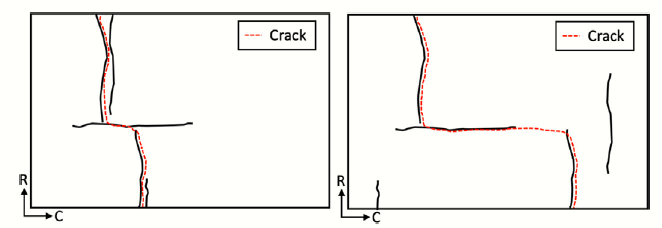
\includegraphics[width=4.3in]{Figures/1-Introduction/same RHF.png}
    \caption{Same hydrides located differently: The same RHF value but different alignment \cite{SIMON2021152817}.}
    \label{fig:RHF_comparison}
\end{figure}
